\documentclass[a4paper,14pt,oneside,openany]{memoir}

\usepackage[left=30mm, right=15mm, top=20mm, bottom=20mm]{geometry}
\pagestyle{plain}
\parindent=1.25cm
\usepackage{indentfirst}

\usepackage{polyglossia}
\setdefaultlanguage[indentfirst=true,forceheadingpunctuation=false]{russian}
\setotherlanguages{english}

\IfFontExistsTF{Times New Roman}
{\setmainfont{Times New Roman}
\newfontfamily\cyrillicfont{Times New Roman}[Script=Cyrillic]}
{\setmainfont[Script=Cyrillic]{FreeSerif}}

\IfFontExistsTF{Courier New}
{\setmonofont{Courier New}
\newfontfamily\cyrillicfonttt{Courier New}[Script=Cyrillic]}
{\setmonofont[Script=Cyrillic]{FreeMono}}

\IfFontExistsTF{Arial}
{\setsansfont{Arial}
\newfontfamily\cyrillicfontsf{Arial}[Script=Cyrillic]}
{\setsansfont[Script=Cyrillic]{FreeSans}}

\setsecnumdepth{subsection}
\renewcommand*{\chapterheadstart}{}
\renewcommand*{\printchaptername}{}
\renewcommand*{\chapnumfont}{\normalfont\bfseries}
\renewcommand*{\afterchapternum}{\hspace{1em}}
\renewcommand*{\printchaptertitle}{\normalfont\bfseries\centering\MakeUppercase}
\setbeforesecskip{20pt}
\setaftersecskip{20pt}
\setsecheadstyle{\raggedright\normalfont\bfseries}
\setbeforesubsecskip{20pt}
\setaftersubsecskip{20pt}
\setsubsecheadstyle{\raggedright\normalfont\bfseries}
\setbeforesubsubsecskip{14pt}
\setaftersubsubsecskip{10pt}
\setsubsubsecheadstyle{\raggedright\normalfont\bfseries}

\addto\captionsrussian{\renewcommand\contentsname{Содержание}}
\setrmarg{2.55em plus1fil}
\renewcommand{\aftertoctitle}{\afterchaptertitle \vspace{-\cftbeforechapterskip}}
\renewcommand*{\cftchapternumwidth}{1.5em}
\renewcommand*{\cftchapterfont}{\normalfont\MakeUppercase}
\renewcommand*{\cftchapterpagefont}{\normalfont}
\renewcommand*{\cftchapterdotsep}{\cftdotsep}
\renewcommand*{\cftdotsep}{1}
\renewcommand*{\cftchapterleader}{\cftdotfill{\cftchapterdotsep}}
\maxtocdepth{subsection}

\tolerance 1414
\hbadness 1414
\emergencystretch 1.5em
\hfuzz 0.3pt
\vfuzz \hfuzz
\clubpenalty=10000
\widowpenalty=10000
\brokenpenalty=4991

\makeatletter
    \def\russian@Alph#1{\ifcase#1\or
       А\or Б\or В\or Г\or Д\or Е\or Ж\or
       И\or К\or Л\or М\or Н\or
       П\or Р\or С\or Т\or У\or Ф\or Х\or
       Ц\or Ш\or Щ\or Э\or Ю\or Я\else\xpg@ill@value{#1}{russian@Alph}\fi}
    \def\russian@alph#1{\ifcase#1\or
       а\or б\or в\or г\or д\or е\or ж\or
       и\or к\or л\or м\or н\or
       п\or р\or с\or т\or у\or ф\or х\or
       ц\or ш\or щ\or э\or ю\or я\else\xpg@ill@value{#1}{russian@alph}\fi}
\makeatother

\usepackage{graphicx, caption, subcaption}
\graphicspath{{images/}}
\captionsetup[figure]{font=small, width=\textwidth, name=Рисунок, justification=centering}
\captionsetup[subfigure]{font=small}
\captionsetup[table]{singlelinecheck=false,font=small,width=\textwidth,justification=justified}
\captiondelim{ - }
\setkeys{Gin}{width=\textwidth}
\renewcommand{\thesubfigure}{\asbuk{subfigure}}
\usepackage[section]{placeins}
\usepackage{float}

\usepackage{hyperref}
\hypersetup{
    colorlinks=true,
    linktoc=all,
    linktocpage=true,
    linkcolor=red,
    citecolor=red,
    urlcolor=red
}

\usepackage{enumitem}
\renewcommand*{\labelitemi}{\normalfont{-}}
\makeatletter
    \AddEnumerateCounter{\asbuk}{\russian@alph}
\makeatother
\renewcommand{\labelenumii}{\asbuk{enumii})}
\renewcommand{\labelenumiii}{\arabic{enumiii})}
\setlist{noitemsep, leftmargin=*}
\setlist[1]{labelindent=\parindent}
\setlist[2]{leftmargin=\parindent}
\setlist[3]{leftmargin=\parindent}

\counterwithout{figure}{chapter}
\counterwithout{equation}{chapter}
\counterwithout{table}{chapter}

\usepackage{longtable,ltcaption}
\usepackage{multirow,makecell}
\usepackage{booktabs}
\usepackage{soulutf8}
\usepackage{icomma}
\usepackage{hyphenat}
\usepackage{textcomp}
\usepackage{amsmath}

\usepackage{listings}
\usepackage{xcolor}

\definecolor{codegreen}{rgb}{0,0.6,0}
\definecolor{codegray}{rgb}{0.5,0.5,0.5}
\definecolor{codepurple}{rgb}{0.58,0,0.82}
\definecolor{backcolour}{rgb}{0.95,0.95,0.92}

\lstdefinestyle{mystyle}{
  backgroundcolor=\color{backcolour},
  commentstyle=\color{codegreen},
  keywordstyle=\color{magenta},
  numberstyle=\tiny\color{codegray},
  stringstyle=\color{codepurple},
  basicstyle=\ttfamily\footnotesize,
  breakatwhitespace=false,
  breaklines=true,
  captionpos=b,
  keepspaces=true,
  numbers=left,
  numbersep=5pt,
  showspaces=false,
  showstringspaces=false,
  showtabs=false,
  tabsize=4,
  frame=single,
  literate=%
    {а}{{а}}1 {б}{{б}}1 {в}{{в}}1 {г}{{г}}1 {д}{{д}}1
    {е}{{е}}1 {ё}{{ё}}1 {ж}{{ж}}1 {з}{{з}}1 {и}{{и}}1
    {й}{{й}}1 {к}{{к}}1 {л}{{л}}1 {м}{{м}}1 {н}{{н}}1
    {о}{{о}}1 {п}{{п}}1 {р}{{р}}1 {с}{{с}}1 {т}{{т}}1
    {у}{{у}}1 {ф}{{ф}}1 {х}{{х}}1 {ц}{{ц}}1 {ч}{{ч}}1
    {ш}{{ш}}1 {щ}{{щ}}1 {ъ}{{ъ}}1 {ы}{{ы}}1
    {ь}{{ь}}1 {э}{{э}}1 {ю}{{ю}}1 {я}{{я}}1
    {А}{{А}}1 {Б}{{Б}}1 {В}{{В}}1 {Г}{{Г}}1 {Д}{{Д}}1
    {Е}{{Е}}1 {Ё}{{Ё}}1 {Ж}{{Ж}}1 {З}{{З}}1 {И}{{И}}1
    {Й}{{Й}}1 {К}{{К}}1 {Л}{{Л}}1 {М}{{М}}1 {Н}{{Н}}1
    {О}{{О}}1 {П}{{П}}1 {Р}{{Р}}1 {С}{{С}}1 {Т}{{Т}}1
    {У}{{У}}1 {Ф}{{Ф}}1 {Х}{{Х}}1 {Ц}{{Ц}}1 {Ч}{{Ч}}1
    {Ш}{{Ш}}1 {Щ}{{Щ}}1 {Ъ}{{Ъ}}1 {Ы}{{Ы}}1
    {Ь}{{Ь}}1 {Э}{{Э}}1 {Ю}{{Ю}}1 {Я}{{Я}}1
    {×}{{$\times$}}1
}
\lstset{style=mystyle}
\renewcommand{\lstlistingname}{Листинг}
\DeclareCaptionLabelSeparator{dash}{ - }
\captionsetup[lstlisting]{singlelinecheck=false,font=small,justification=centering,labelsep=dash}

\begin{document}
\thispagestyle{empty}

\begin{center}
    МИНИСТЕРСТВО ЦИФРОВОГО РАЗВИТИЯ, СВЯЗИ И МАССОВЫХ КОММУНИКАЦИЙ \\ РОССИЙСКОЙ ФЕДЕРАЦИИ

    \vspace{20pt}

    Федеральное государственное бюджетное образовательное учреждение \\ высшего образования \\
    \textquotedbl{}Сибирский государственный университет телекоммуникаций и информатики\textquotedbl{}

    \vspace{20pt}

    Кафедра телекоммуникационных систем и вычислительных средств \\ (ТС и ВС)
\end{center}

\vfill

\begin{center}
    ОТЧЁТ \\
    о практической работе №1 \\
    по дисциплине \\
    \textit{\textquotedbl{}Основы систем мобильной связи\textquotedbl{}}

    \vspace{20pt}

    по теме: \\
    \uppercase{Временная и частотная формы сигналов. Преобразования Фурье. Дискретизация сигналов}
\end{center}

\vfill

    \noindent Студент: \\
    \textit{Группа ИКС-433 \hfill Воробьёв Д. А.}

    \vspace{20pt}

    \noindent Преподаватель: \\
    \textit{заведующий кафедрой \hfill Дроздова В. Г.}

\vfill

\begin{center}
    Новосибирск 2026 г.
\end{center}

\newpage
\setcounter{page}{2}
\OnehalfSpacing*

\tableofcontents*

\chapter{Практическая работа №1. Временная и частотная формы сигналов. Преобразования Фурье. Дискретизация сигналов}
\label{ch:lab1}

\section{Цель и задачи работы}

Цель работы: изучить влияние частоты дискретизации и разрядности АЦП на частотные характеристики сигнала, освоить дискретные преобразования Фурье для переходов между временным и частотным представлениями сигналов.

Задачи работы:

\begin{itemize}
  \item сгенерировать и визуализировать непрерывный сигнал по варианту, определить максимальную частоту в его спектре и минимальную частоту дискретизации по теореме Котельникова;
  \item оцифровать сигнал, выполнить прямое дискретное преобразование Фурье, оценить ширину спектра и объём памяти для хранения отсчётов;
  \item восстановить сигнал по отсчётам и оценить сходство с оригиналом, повторить эксперимент при частоте дискретизации, увеличенной в 4 раза;
  \item записать голос, определить его максимальную частоту и частоту дискретизации записи, оценить влияние неверно выбранной частоты дискретизации на звук и на спектр;
  \item оценить влияние разрядности АЦП на спектр сигнала и среднюю ошибку квантования.
\end{itemize}

\section{Краткие теоретические сведения}

\subsection{Дискретизация и теорема Котельникова}

Чтобы обрабатывать сигнал на компьютере, непрерывную функцию $x(t)$ заменяют набором её значений (отсчётов) в моменты времени, кратные периоду дискретизации $T_s = 1/f_s$:

\begin{equation*}
x[n] = x(nT_s) = x\left(\frac{n}{f_s}\right), \quad n = 0, 1, 2, \dots
\end{equation*}

Теорема Котельникова: сигнал со спектром, ограниченным частотой $f_{max}$, можно без потерь восстановить по его отсчётам, если частота дискретизации строго больше удвоенной максимальной частоты:

\begin{equation*}
f_s > 2 f_{max}.
\end{equation*}

Если условие не выполняется, высокие частоты сигнала \textquotedbl{}складываются\textquotedbl{} с низкими, и исходный сигнал восстановить нельзя.

\subsection{Квантование и АЦП}

Аналого-цифровой преобразователь (АЦП) выполняет дискретизацию по времени и квантование по уровню: амплитуду каждого отсчёта округляют до одного из $2^n$ возможных значений, где $n$ - разрядность АЦП. Шаг квантования при размахе сигнала от $x_{min}$ до $x_{max}$ равен

\begin{equation*}
\Delta = \frac{x_{max} - x_{min}}{2^n - 1},
\end{equation*}

а ошибка квантования (разница между исходным и округлённым значением) не превышает $\Delta / 2$. Чем больше разрядов у АЦП, тем меньше ошибка квантования. Для хранения одного отсчёта нужно $n$ бит, поэтому увеличение разрядности и частоты дискретизации увеличивает и объём памяти.

\subsection{Дискретное преобразование Фурье}

Любой сигнал можно представить суммой гармоник с разными частотами, амплитудами и фазами. Прямое преобразование Фурье (ППФ) переводит временное представление сигнала в частотное, обратное преобразование Фурье (ОПФ) выполняет обратный переход. Для дискретного сигнала из $N$ отсчётов прямое преобразование имеет вид (1.8):

\begin{equation*}
F(x) = \sum_{n=0}^{N-1} f(n)\, e^{-j 2\pi \frac{x n}{N}},
\end{equation*}

а обратное (1.9):

\begin{equation*}
f(n) = \frac{1}{N} \sum_{x=0}^{N-1} F(x)\, e^{j 2\pi \frac{x n}{N}}.
\end{equation*}

Результат ППФ - массив из $N$ комплексных чисел. Номер элемента $k$ соответствует частоте $f_k = k f_s / N$, амплитуда гармоники равна $|F(k)|/N$, фаза - аргументу комплексного числа. Для вещественного сигнала вторая половина спектра является зеркальным отражением первой, поэтому ширину спектра оценивают по первой половине (до $N/2$).

\subsection{Быстрое преобразование Фурье}

Прямое вычисление по формуле требует порядка $N^2$ операций. Быстрое преобразование Фурье (БПФ) группирует слагаемые с одинаковыми множителями и вычисляет то же преобразование за порядка $N \log_2 N$ операций, при этом длина входного массива обычно равна $N = 2^k$. БПФ используется в модемах мобильных устройств, а в работе - для спектра длинной записи голоса.

\subsection{Ширина спектра}

Шириной спектра называют диапазон частот, в котором сигнал имеет заметную амплитуду. Из-за ошибок округления отсутствующие в сигнале частоты получаются не точно нулевыми, поэтому значимыми считают частоты, амплитуда которых превышает заданный порог.

\section{Исходные данные}

Вариант 5. Непрерывная периодическая функция:

\begin{equation*}
y(t) = \cos\left(2\pi f t + \frac{\pi}{3}\right) + \sin(4\pi f t), \quad f = 4.
\end{equation*}

Сигнал рассматривается на интервале длительностью 1 с, для имитации непрерывного сигнала используется сетка в 1024 отсчёта на секунду. Запись голоса: файл \texttt{voice.wav}, моно, частота дискретизации 44100 Гц, длительность 6,14 с.

Расчёты выполнены на языке Python с использованием библиотек NumPy, SciPy, Matplotlib и icecream. Ниже приведены подключаемые функции проекта и параметры сетки времени.

\begin{lstlisting}[language=Python, caption={Подключение библиотек и функций проекта}]
import sys
from pathlib import Path

sys.path.insert(0, str(Path.cwd().parent))

from icecream import ic

import numpy as np
import utils.debug
from matplotlib.axes import Axes

from utils.complex_numbers import to_polar, to_rect
from utils.harmonic import (
    get_harmonic_oscillation,
    get_period,
    get_phase_time_shift,
    get_phase_at,
)
from utils.spectrum import get_spectrum, get_spectrum_width
from utils.fourier import discrete_fourier_transform
from utils.quantize import quantize, quantize_np
from utils.plotting import show_multi_plot, show_plot
from utils.sampling import get_linspace
from scipy.io import wavfile
from IPython.display import Audio
\end{lstlisting}

\begin{lstlisting}[language=Python, caption={Параметры времени и сетка отсчётов}]
sampling_frequency = 1024
start = 0
stop =  1
t = get_linspace(start=start, stop=stop, fs=sampling_frequency)
\end{lstlisting}


\section{Ход работы}

\subsection{Задание 1}

Необходимо сгенерировать и визуализировать (вывести на график) непрерывный сигнал, в соответствии с вариантом (таблица 1.1). Номер варианта - порядковый номер в журнале группы.

\begin{lstlisting}[language=Python, caption={Генерация и построение непрерывного сигнала}]
frequency = 4

ic(frequency)
ic(sampling_frequency)

y_1 = get_harmonic_oscillation(1, frequency, np.pi/3, wave=np.cos)(t)
y_2 = get_harmonic_oscillation(1, 2*frequency, 0, wave=np.sin)(t)
y = y_1 + y_2  # 5 вариант

show_plot(
    t=t,
    func_val=y,
    title="cos(2*pi*f*t + pi/3) + sin(4*pi*f*t)",
)
\end{lstlisting}

\begin{lstlisting}[language={}, numbers=none, backgroundcolor=\color{white}, caption={Результат выполнения: генерация и построение непрерывного сигнала}]
ic| frequency: 4
ic| sampling_frequency: 1024
\end{lstlisting}

\begin{figure}[H]
\centering
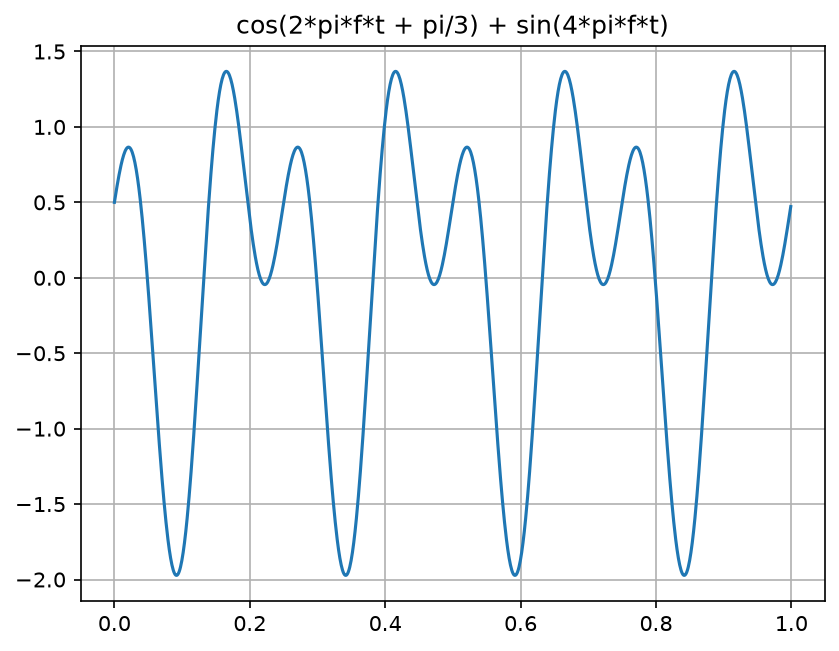
\includegraphics[width=0.8\textwidth]{c04_0.png}
\caption{Непрерывный сигнал варианта 5}
\label{fig:c04_0}
\end{figure}

\subsubsection{Вывод}

Сигнал состоит из двух гармоник и повторяется каждую 1/4 секунды (период медленной гармоники 4 Гц), на графике это 4 одинаковых периода. Размах сигнала примерно от -2 до 1,4.

\subsection{Задание 2}

Определить максимальную частоту в спектре данного сигнала.

\textbf{Расчёт.} Сигнал (варианта 5) состоит из двух гармоник:

\begin{equation*}
y(t) = \cos(2\pi f t + \tfrac{\pi}{3}) + \sin(4\pi f t),\quad f = 4\ \text{Гц}
\end{equation*}

Частота каждой гармоники:

\begin{itemize}
\item $\cos(2\pi f t + \tfrac{\pi}{3})$: частота $f_1 = f = 4$ Гц;
\item $\sin(4\pi f t) = \sin(2\pi \cdot 2f \cdot t)$: частота $f_2 = 2f = 8$ Гц.
\end{itemize}

Спектр сигнала состоит из этих двух частот, поэтому максимальная частота - наибольшая из них:

\begin{equation*}
f_{max} = \max(f_1, f_2) = 2f = 2 \cdot 4 = 8\ \text{Гц}
\end{equation*}

\begin{lstlisting}[language=Python, caption={Максимальная частота сигнала}]
max_freq = frequency * 2
ic(max_freq);
\end{lstlisting}

\begin{lstlisting}[language={}, numbers=none, backgroundcolor=\color{white}, caption={Результат выполнения: максимальная частота сигнала}]
ic| max_freq: 8
\end{lstlisting}

\subsection{Задание 3}

Определить минимальную необходимую частоту дискретизации полученного сигнала (теорема Котельникова).

\begin{lstlisting}[language=Python, caption={Частота дискретизации по Котельникову}]
# min_freq_kotelnikov = max_freq * 2
min_freq_kotelnikov = max_freq * 4

ic(max_freq)
ic(min_freq_kotelnikov);
\end{lstlisting}

\begin{lstlisting}[language={}, numbers=none, backgroundcolor=\color{white}, caption={Результат выполнения: частота дискретизации по Котельникову}]
ic| max_freq: 8
ic| min_freq_kotelnikov: 32
\end{lstlisting}

\textbf{Примечание.} По теореме Котельникова $f_s$ должна быть \textit{строго больше} $2 f_{max}$. При $f_s = 2 f_{max} = 16$ Гц отсчёты восьмигерцовой гармоники $\sin(4\pi f t)$ попадают ровно в нули синуса, и она теряется.

Брать произвольное $f_s > 16$ Гц (например, 17 или 20) неудобно: сетка 1024 точки на 1 секунду не делится на такое число нацело, поэтому шаг \texttt{step} получается дробным и отсчёты получаются неравномерными.

Поэтому выбрано $f_s = 4 f_{max} = 32$ Гц: это ближайшая степень двойки выше минимума, она делит 1024 нацело (шаг 32), отсчёты равномерны.

\subsection{Задание 4}

Оцифровать сигнал с полученной частотой дискретизации, выбрав требуемое число отсчетов сигнала на длительности 1 секунда, сохранить полученные значения в массив, пока не озадачиваясь разрядностью АЦП, просто выбранные с частотой дискретизации значения с теми уровнями, которые имеет функция в полученных точках.

\begin{lstlisting}[language=Python, caption={Дискретизация сигнала}]
step = len(y) // int(min_freq_kotelnikov * (stop - start))

# прореживая по шагу step
y_sampled = y[::step]
t_sampled = t[::step]

ic(y_sampled)
ic(t_sampled);
\end{lstlisting}

\begin{lstlisting}[language={}, numbers=none, backgroundcolor=\color{white}, caption={Результат выполнения: дискретизация сигнала}]
ic| y_sampled: array([ 0.5       ,  0.74118095, -0.8660254 , -1.96592583, -0.5       ,
                       1.25881905,  0.8660254 , -0.03407417,  0.5       ,  0.74118095,
                      -0.8660254 , -1.96592583, -0.5       ,  1.25881905,  0.8660254 ,
                      -0.03407417,  0.5       ,  0.74118095, -0.8660254 , -1.96592583,
                      -0.5       ,  1.25881905,  0.8660254 , -0.03407417,  0.5       ,
                       0.74118095, -0.8660254 , -1.96592583, -0.5       ,  1.25881905,
                       0.8660254 , -0.03407417])
ic| t_sampled: array([0.     , 0.03125, 0.0625 , 0.09375, 0.125  , 0.15625, 0.1875 ,
                      0.21875, 0.25   , 0.28125, 0.3125 , 0.34375, 0.375  , 0.40625,
                      0.4375 , 0.46875, 0.5    , 0.53125, 0.5625 , 0.59375, 0.625  ,
                      0.65625, 0.6875 , 0.71875, 0.75   , 0.78125, 0.8125 , 0.84375,
                      0.875  , 0.90625, 0.9375 , 0.96875])
\end{lstlisting}

\begin{lstlisting}[language=Python, caption={Построение сигнала и отсчётов}]
def draw_samples(ax: Axes) -> None:
    ax.stem(t_sampled, y_sampled, linefmt="r-", markerfmt="ro", basefmt=" ")

show_plot(
    t=t,
    func_val=y,
    title="Сигнал и отсчеты",
    on_axes=draw_samples,
)
\end{lstlisting}

\begin{figure}[H]
\centering
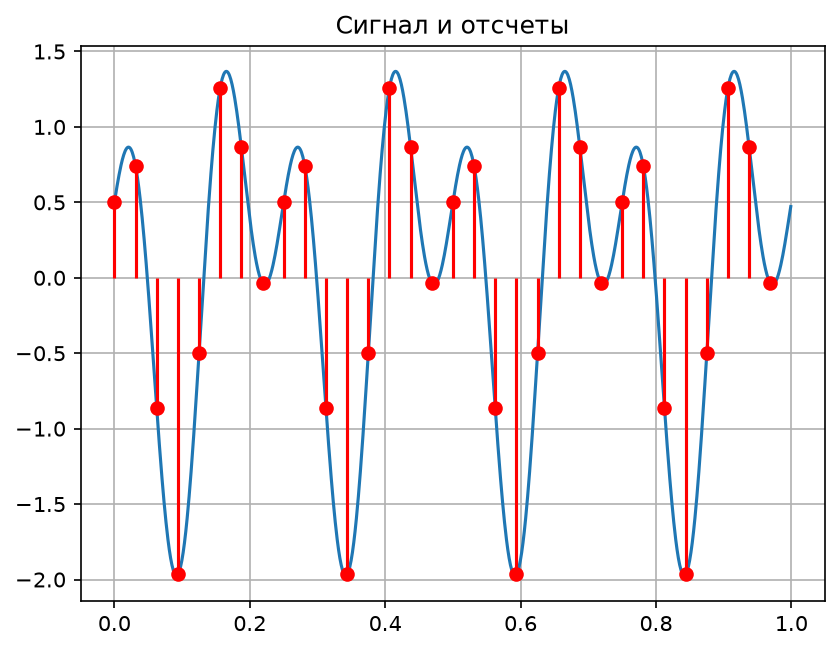
\includegraphics[width=0.8\textwidth]{c14_0.png}
\caption{Сигнал и отсчёты, $f_s = 32$ Гц}
\label{fig:c14_0}
\end{figure}

\begin{lstlisting}[language=Python, caption={Построение сигнала по отсчётам}]
show_plot(
    t=t_sampled,
    func_val=y_sampled,
    title=f"частота по Котельникову = {min_freq_kotelnikov}",
)
\end{lstlisting}

\begin{figure}[H]
\centering
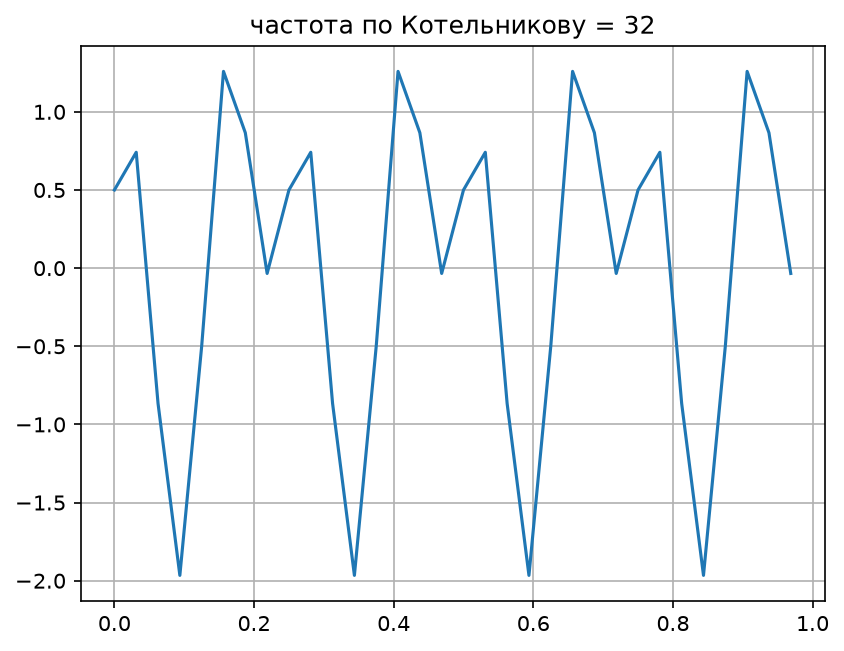
\includegraphics[width=0.8\textwidth]{c15_0.png}
\caption{Сигнал по отсчётам, $f_s = 32$ Гц}
\label{fig:c15_0}
\end{figure}

\subsubsection{Вывод}

Взяли каждый 32-й отсчёт из 1024, получилось 32 отсчёта на секунду, то есть частота дискретизации 32 Гц. Обе гармоники сигнала по ним различимы.

\subsection{Задание 5}

Выполнить прямое дискретное преобразование Фурье для массива временных отсчетов сигнала и оценить ширину данного спектра. А также объем памяти, требуемый для хранения данного массива (тип переменных в массиве - на ваше усмотрение, float, int и пр.).

\subsubsection{Что делает преобразование Фурье}

Мы смотрим на сигнал и спрашиваем: Из каких гармоник он состоит?

Для этого мы используем прямое преобразование Фурье по формуле:

\begin{equation*}
F(x) = \sum_{n=0}^{N-1} f(n)\, e^{-j 2\pi \frac{x n}{N}},
\end{equation*}

где $N$ - размерность преобразования Фурье, $F(x)$ - сигнал в частотной области и $f(n)$ - дискретизированный сигнал во временной области.

Листинг функции \texttt{utils/fourier.py}:

\begin{lstlisting}[language=Python, caption={Функция прямого ДПФ (utils/fourier.py)}]
def discrete_fourier_transform(x: np.ndarray) -> np.ndarray:
    N = len(x)
    X = []
    for k in range(N):
        s = 0
        for n in range(N):
            s += x[n] * np.exp(-2j * np.pi * k * n / N)
        X.append(s)

    return np.array(X)
\end{lstlisting}

\textbf{Что она возвращает.} Массив из \texttt{N} комплексных чисел (столько же, сколько отсчётов на входе). Число номер \texttt{k} относится к частоте номер \texttt{k}. Комплексное число хранит сразу две вещи: амплетуду и фазу.

\textbf{Как достать нужное:}

\begin{center}
\begin{tabular}{|p{4.6cm}|p{5.6cm}|p{4cm}|}
\hline
Что нужно & Как получить & В коде \\
\hline
Частота \texttt{k}-й гармоники & номер умножить на шаг частоты & \texttt{k * fs / N} \\
\hline
Амплитуда (сила волны) & модуль комплексного числа, делённый на \texttt{N} & \texttt{np.abs(X) / N} \\
\hline
Фаза (сдвиг) & угол комплексного числа & \texttt{np.angle(X)} \\
\hline
\end{tabular}
\end{center}

Из-за ошибок округления "ненужные" частоты получаются не ровно 0, а очень маленькими числами. Поэтому мы задаём порог \texttt{threshold} и считаем значимыми только те частоты, где амплитуда больше него.

\textbf{Что считать шириной спектра.} Это диапазон частот, в котором есть сигнал. Есть два способа считать:

\begin{itemize}
\item \texttt{max - min} - от самой низкой до самой высокой значимой частоты (у нас 4 и 8 Гц, получится 4 Гц). Так считают для полосовых сигналов, у которых спектр где-то посередине.
\item \texttt{max} - от нуля до самой высокой частоты (получится 8 Гц). Так считают для сигналов в основной полосе, которые мы оцифровываем с нуля.
\end{itemize}

Я взял второй вариант: \texttt{f\_max = 8} Гц.

\begin{lstlisting}[language=Python, caption={Прямое ДПФ и оценка ширины спектра}]
y_dft = discrete_fourier_transform(y_sampled)
N = len(y_dft)
freqs = np.arange(N) * (min_freq_kotelnikov / N)
amp = np.abs(y_dft) / N

ic(freqs)
ic(amp)

threshold = 1e-6 # порог для выделения значимых частот
half = N // 2 + 1  # без зеркальной части
significant = np.array([freqs[k] for k in range(half) if amp[k] > threshold])
# spectrum_width = significant.max() - significant.min()
spectrum_width = significant.max()

ic(spectrum_width);
\end{lstlisting}

\begin{lstlisting}[language={}, numbers=none, backgroundcolor=\color{white}, caption={Результат выполнения: прямое ДПФ и оценка ширины спектра}]
ic| freqs: array([ 0.,  1.,  2.,  3.,  4.,  5.,  6.,  7.,  8.,  9., 10., 11., 12.,
                  13., 14., 15., 16., 17., 18., 19., 20., 21., 22., 23., 24., 25.,
                  26., 27., 28., 29., 30., 31.])
ic| amp: array([2.77555756e-17, 7.39993399e-17, 3.16461231e-17, 3.51614705e-16,
                5.00000000e-01, 3.94695830e-16, 1.97240692e-16, 1.54996458e-16,
                5.00000000e-01, 1.13698104e-16, 2.95841644e-16, 2.62533797e-16,
                3.64355492e-16, 8.13652846e-16, 5.08091498e-16, 3.89364649e-16,
                1.83568042e-15, 6.64082938e-16, 6.87560229e-16, 4.47316182e-16,
                3.45556987e-16, 3.87944218e-16, 3.95369749e-16, 1.23716373e-15,
                5.00000000e-01, 6.70588694e-16, 5.00919297e-16, 1.54605159e-15,
                5.00000000e-01, 1.29373207e-15, 6.35261403e-16, 3.62091088e-16])
ic| spectrum_width: np.float64(8.0)
\end{lstlisting}

\begin{lstlisting}[language=Python, caption={Построение полного амплитудного спектра}]
show_plot(
    t=freqs,
    func_val=amp,
    is_stem=True,
    title="Амплитудный спектр, все N гармоник (зеркальная часть)",
)
\end{lstlisting}

\begin{figure}[H]
\centering
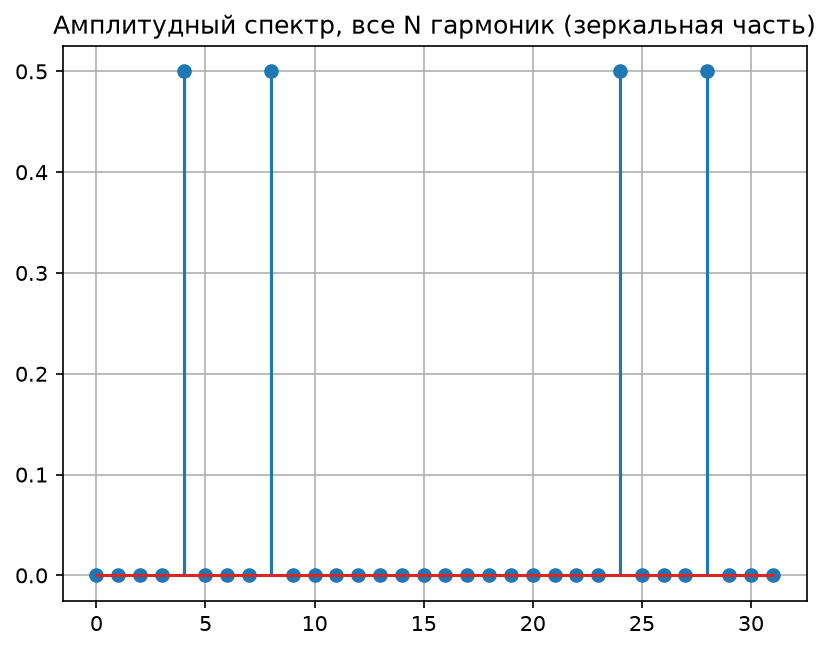
\includegraphics[width=0.8\textwidth]{c21_0.png}
\caption{Амплитудный спектр, все $N$ гармоник (с зеркальной частью)}
\label{fig:c21_0}
\end{figure}

\begin{lstlisting}[language=Python, caption={Построение спектра без зеркальной части}]
def draw_threshold(ax: Axes) -> None:
    ax.axhline(threshold, color="gray", linestyle="--", label="порог")
    ax.axvline(spectrum_width, color="r", linestyle=":", label="ширина спектра")
    ax.legend()

show_plot(
    t=freqs[:half],
    func_val=amp[:half],
    is_stem=True,
    title="Амплитудный спектр без зеркальной части",
    on_axes=draw_threshold,
)
\end{lstlisting}

\begin{figure}[H]
\centering
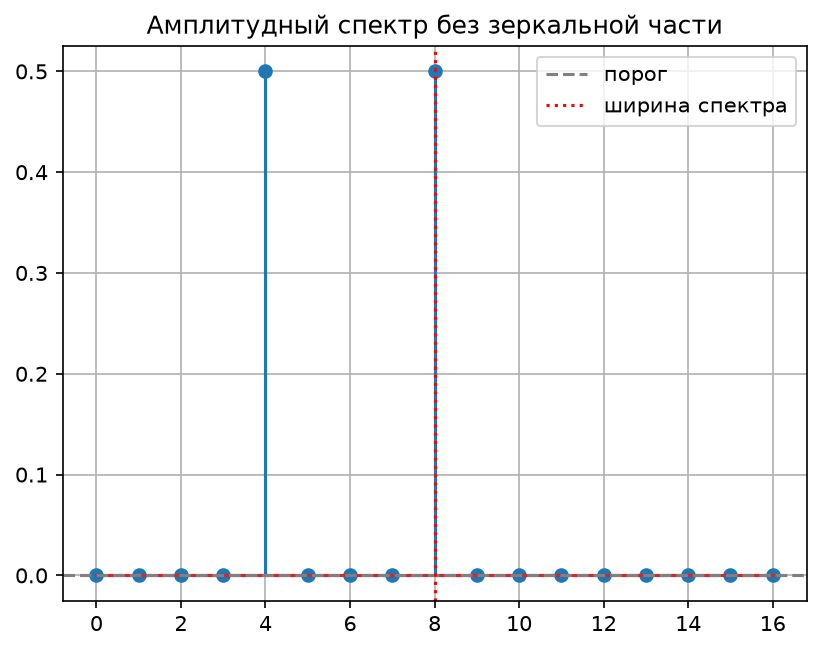
\includegraphics[width=0.8\textwidth]{c22_0.png}
\caption{Амплитудный спектр без зеркальной части}
\label{fig:c22_0}
\end{figure}

\subsubsection{Объём памяти для y\_sampled}

\begin{lstlisting}[language=Python, caption={Объём памяти массива отсчётов}]
ic(y_sampled.dtype)   # float64 - 64 бита / 8 байт на отсчёт
ic(y_sampled.size)    # 32 отсчёта (fs = 32 Гц на 1 с)
ic(y_sampled.nbytes);  # 256 байт = 32 * 8
\end{lstlisting}

\begin{lstlisting}[language={}, numbers=none, backgroundcolor=\color{white}, caption={Результат выполнения: объём памяти массива отсчётов}]
ic| y_sampled.dtype: dtype('float64')
ic| y_sampled.size: 32
ic| y_sampled.nbytes: 256
\end{lstlisting}

\subsubsection{Объём памяти для y\_dft}

\begin{lstlisting}[language=Python, caption={Объём памяти массива спектра}]
ic(y_dft.dtype)   # complex128 - 128 бит / 16 байт на отсчёт
ic(y_dft.size)    # 32 отсчёта (fs = 32 Гц на 1 с)
ic(y_dft.nbytes); # 512 байт = 32 * 16
\end{lstlisting}

\begin{lstlisting}[language={}, numbers=none, backgroundcolor=\color{white}, caption={Результат выполнения: объём памяти массива спектра}]
ic| y_dft.dtype: dtype('complex128')
ic| y_dft.size: 32
ic| y_dft.nbytes: 512
\end{lstlisting}

\subsubsection{Вывод}

\begin{itemize}
\item В спектре две гармоники: на 4 Гц и на 8 Гц.
\item Остальные частоты равны нулю (с точностью до ошибок округления), поэтому ширина спектра равна 8 Гц, как и максимальная частота из задания 2.
\item Для хранения 32 отсчётов в \texttt{float64} нужно 256 байт, для их спектра в \texttt{complex128} - 512 байт.
\end{itemize}

\subsection{Задание 6}

Восстановите оригинальный аналоговый сигнал по массиву имеющихся у вас отсчетов, соединив их непрерывной линией и оцените визуальное сходство оригинального сигнала и восстановленного после оцифровки.

\begin{lstlisting}[language=Python, caption={Восстановление сигнала по отсчётам}]
show_multi_plot(
    t=[t, t_sampled],
    func_vals=[y, y_sampled],
    labels=["оригинал", "восстановленный"],
    title=f"Восстановление по отсчётам, fs = {min_freq_kotelnikov}",
)
\end{lstlisting}

\begin{figure}[H]
\centering
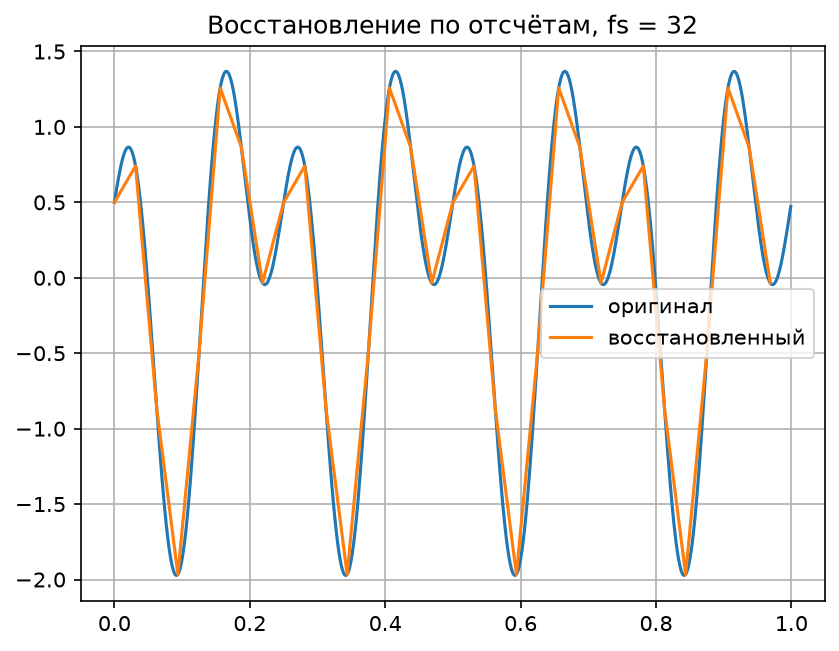
\includegraphics[width=0.8\textwidth]{c29_0.png}
\caption{Восстановление сигнала по отсчётам, $f_s = 32$ Гц}
\label{fig:c29_0}
\end{figure}

\begin{lstlisting}[language=Python, caption={Ошибка восстановления}]
y_restored = np.interp(t, t_sampled, y_sampled)
mask = t <= t_sampled[-1]  # только там, где есть отсчёты с обеих сторон
restore_error = np.mean(np.abs(y[mask] - y_restored[mask]))

ic(restore_error);
\end{lstlisting}

\begin{lstlisting}[language={}, numbers=none, backgroundcolor=\color{white}, caption={Результат выполнения: ошибка восстановления}]
ic| restore_error: np.float64(0.13764728860662287)
\end{lstlisting}

\subsubsection{Вывод}

Восстановленный сигнал повторяет форму оригинала, но в виде ломаной линии, потому что на период самой быстрой гармоники (8 Гц) приходится всего 4 отсчёта. Частота по Котельникову гарантирует, что информация о сигнале сохранена, но простое соединение точек прямыми восстанавливает его грубо.

\subsection{Задание 7}

Увеличьте частоту дискретизации в 4 раза и проделайте задания из п.4-6.

\subsubsection{Пункт 4 (fs × 4)}

\begin{lstlisting}[language=Python, caption={Дискретизация с частотой, увеличенной в 4 раза}]
min_freq_4x = min_freq_kotelnikov * 4
step_4x = len(y) // int(min_freq_4x * (stop - start))

y_sampled_4x = y[::step_4x]
t_sampled_4x = t[::step_4x]

ic(min_freq_4x)
ic(step_4x)
ic(y_sampled_4x.size);
\end{lstlisting}

\begin{lstlisting}[language={}, numbers=none, backgroundcolor=\color{white}, caption={Результат выполнения: дискретизация с частотой, увеличенной в 4 раза}]
ic| min_freq_4x: 128
ic| step_4x: 8
ic| y_sampled_4x.size: 128
\end{lstlisting}

\begin{lstlisting}[language=Python, caption={Построение сигнала и отсчётов при увеличенной в 4 раза частоте}]
def draw_samples_4x(ax: Axes) -> None:
    ax.stem(t_sampled_4x, y_sampled_4x, linefmt="r-", markerfmt="ro", basefmt=" ")

show_plot(
    t=t,
    func_val=y,
    title="Сигнал и отсчеты, fs × 4",
    on_axes=draw_samples_4x,
)
\end{lstlisting}

\begin{figure}[H]
\centering
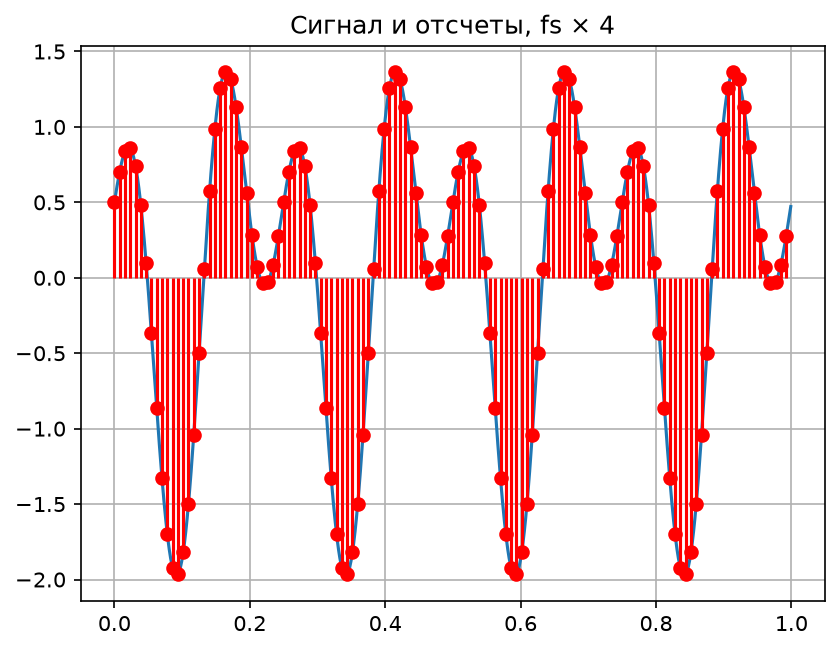
\includegraphics[width=0.8\textwidth]{c35_0.png}
\caption{Сигнал и отсчёты, $f_s = 128$ Гц}
\label{fig:c35_0}
\end{figure}

\subsubsection{Пункт 5 (fs × 4)}

\begin{lstlisting}[language=Python, caption={ДПФ и ширина спектра при увеличенной в 4 раза частоте}]
y_dft_4x = discrete_fourier_transform(y_sampled_4x)
N_4x = len(y_dft_4x)
freqs_4x = np.arange(N_4x) * (min_freq_4x / N_4x)
amp_4x = np.abs(y_dft_4x) / N_4x

half_4x = N_4x // 2 + 1  # без зеркальной части
significant_4x = np.array([freqs_4x[k] for k in range(half_4x) if amp_4x[k] > threshold])
spectrum_width_4x = significant_4x.max()

ic(spectrum_width_4x)
ic(y_sampled_4x.nbytes);
\end{lstlisting}

\begin{lstlisting}[language={}, numbers=none, backgroundcolor=\color{white}, caption={Результат выполнения: дПФ и ширина спектра при увеличенной в 4 раза частоте}]
ic| spectrum_width_4x: np.float64(8.0)
ic| y_sampled_4x.nbytes: 1024
\end{lstlisting}

\begin{lstlisting}[language=Python, caption={Спектр при увеличенной в 4 раза частоте}]
def draw_threshold_4x(ax: Axes) -> None:
    ax.axhline(threshold, color="gray", linestyle="--", label="порог")
    ax.axvline(spectrum_width_4x, color="r", linestyle=":", label="ширина спектра")
    ax.legend()

show_plot(
    t=freqs_4x[:half_4x],
    func_val=amp_4x[:half_4x],
    is_stem=True,
    title="Амплитудный спектр без зеркальной части, fs × 4",
    on_axes=draw_threshold_4x,
)
\end{lstlisting}

\begin{figure}[H]
\centering
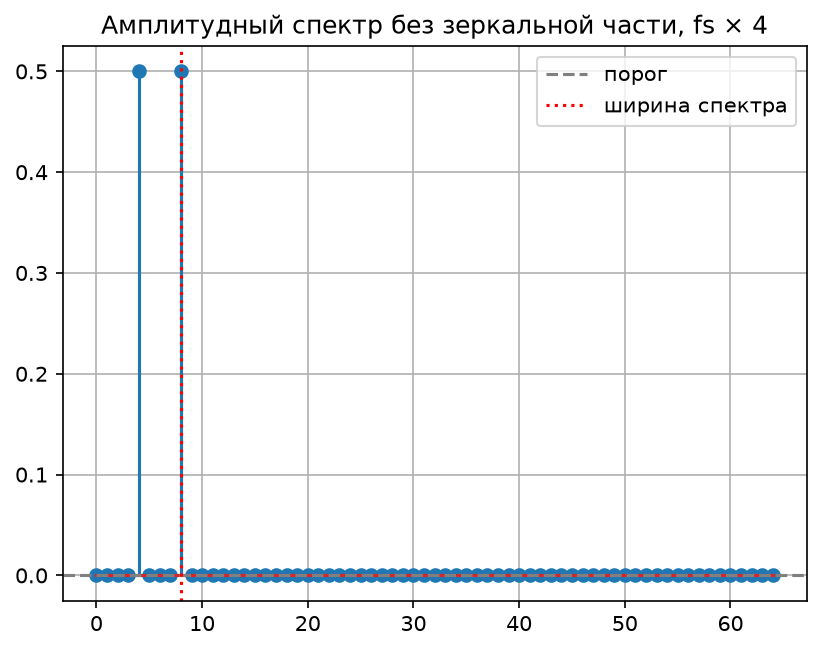
\includegraphics[width=0.8\textwidth]{c38_0.png}
\caption{Амплитудный спектр без зеркальной части, $f_s = 128$ Гц}
\label{fig:c38_0}
\end{figure}

\subsubsection{Пункт 6 (fs × 4)}

\begin{lstlisting}[language=Python, caption={Восстановление по отсчётам при увеличенной в 4 раза частоте}]
show_multi_plot(
    t=[t, t_sampled_4x],
    func_vals=[y, y_sampled_4x],
    labels=["оригинал", "восстановленный"],
    title=f"Восстановление по отсчётам, fs = {min_freq_4x}",
)
\end{lstlisting}

\begin{figure}[H]
\centering
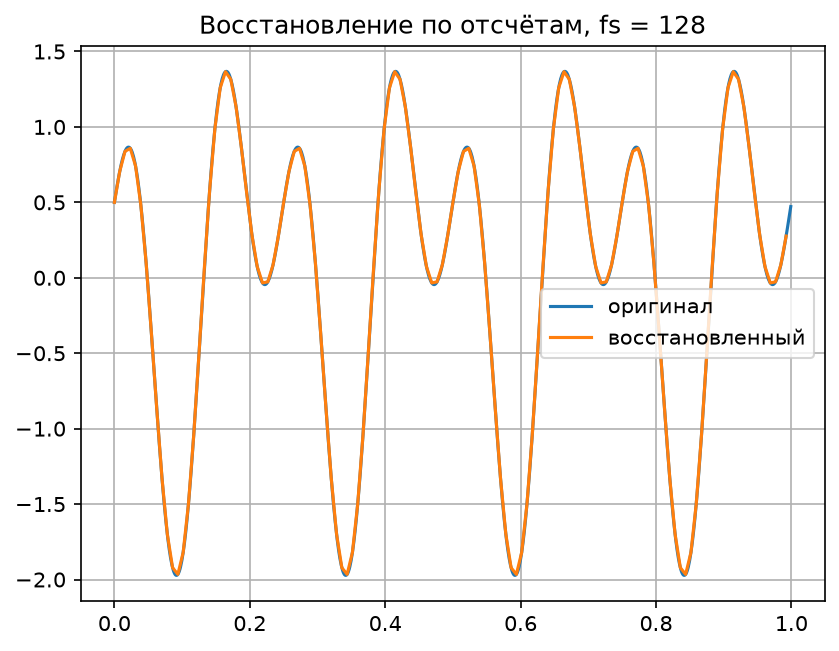
\includegraphics[width=0.8\textwidth]{c40_0.png}
\caption{Восстановление сигнала по отсчётам, $f_s = 128$ Гц}
\label{fig:c40_0}
\end{figure}

\begin{lstlisting}[language=Python, caption={Ошибка восстановления при увеличенной в 4 раза частоте}]
y_restored_4x = np.interp(t, t_sampled_4x, y_sampled_4x)
mask_4x = t <= t_sampled_4x[-1]  # только там, где есть отсчёты с обеих сторон
restore_error_4x = np.mean(np.abs(y[mask_4x] - y_restored_4x[mask_4x]))

ic(restore_error_4x);
\end{lstlisting}

\begin{lstlisting}[language={}, numbers=none, backgroundcolor=\color{white}, caption={Результат выполнения: ошибка восстановления при увеличенной в 4 раза частоте}]
ic| restore_error_4x: np.float64(0.008166292192515932)
\end{lstlisting}

\subsubsection{Что изменилось}

\begin{itemize}
\item Отсчётов стало в 4 раза больше, поэтому и памяти нужно в 4 раза больше.
\item Восстановленная линия стала гораздо ближе к оригиналу.
\end{itemize}

\subsection{Задание 8}

Запишите аудиофайл со своим голосом (например, в формате wav). Проанализируйте визуально спектр голоса, используя, например, приложение Audacity (вкладки Анализ $\rightarrow$ График спектра). Определите максимальную частоту в спектре данного сигнала и выберите требуемую для оцифровки частоту дискретизации.

Запись голоса \texttt{voice.wav} (6,14 с, 44100 Гц, моно).

\begin{figure}[H]
\centering
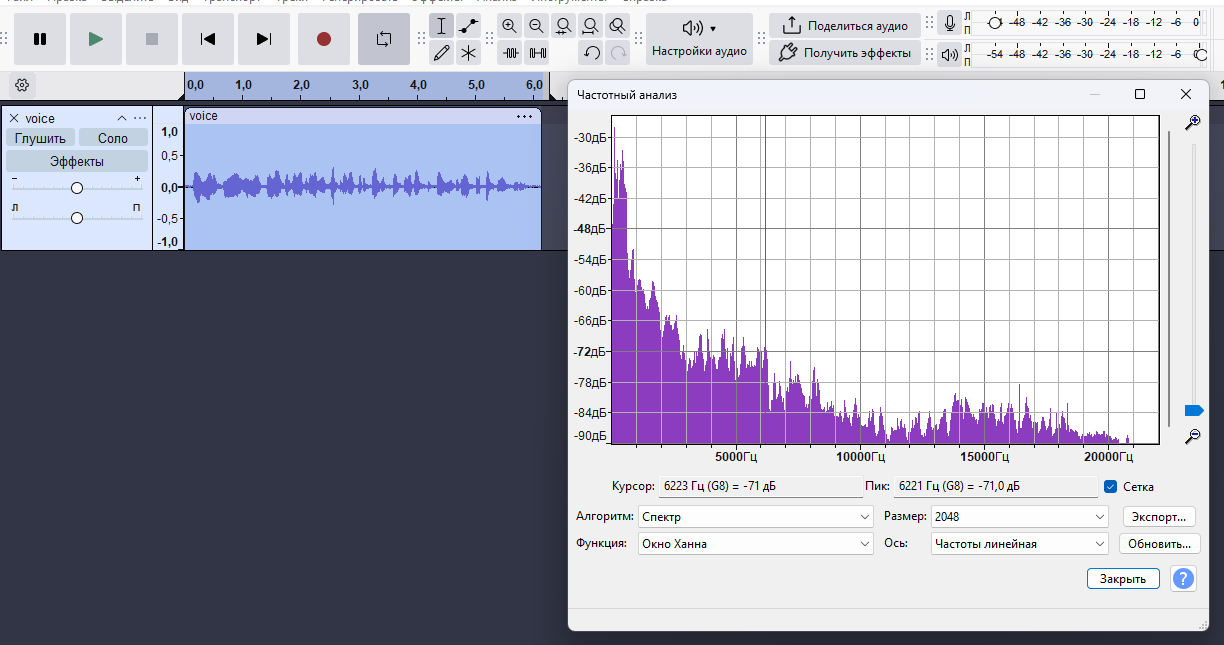
\includegraphics[width=0.8\textwidth]{Screenshot_1.png}
\caption{Временное и частотное представление голоса в Audacity}
\label{fig:Screenshot_1}
\end{figure}

\subsubsection{Максимальная частота и частота дискретизации}

На графике видно, что почти вся энергия голоса сосредоточена в низких частотах, а дальше спектр спадает. Заметный голосовой спектр заканчивается примерно на частоте $f_{max} \approx 6200$ Гц (курсор на: 6223 Гц, -71 дБ). Дальше идёт уровень шума, там самого голоса уже нет.

По теореме Котельникова частота дискретизации должна быть строго больше удвоенной максимальной частоты:

\begin{equation*}
f_s > 2 f_{max} = 2 \cdot 6200 = 12400\ \text{Гц}
\end{equation*}

Значит, для оцифровки такого голоса достаточно, например, $f_s = 16000$ Гц.

\subsection{Задание 9}

Используя библиотеки работы со звуком Matlab (или Pyton) проанализируйте имеющуюся у вас запись голоса. Считайте аудиофайл с помощью функции Matlab (файл с голосом должен лежать в рабочей директории Matlab):

\begin{lstlisting}[language=Matlab]
[y, Fs] = audioread('voice.wav');
\end{lstlisting}

где y - это массив отсчетов голоса, а Fs - частота дискретизации или семплирования, которая определяется в Matlab для данного файла.

\begin{lstlisting}[language=Python, caption={Чтение файла voice.wav}]
Fs, y_voice = wavfile.read("voice.wav")

if y_voice.ndim > 1:
    y_voice = y_voice[:, 0]

if np.issubdtype(y_voice.dtype, np.integer):
    y_voice = y_voice / np.iinfo(y_voice.dtype).max  # приводим к диапазону -1..1

ic(Fs)
ic(y_voice.size);
\end{lstlisting}

\begin{lstlisting}[language={}, numbers=none, backgroundcolor=\color{white}, caption={Результат выполнения: чтение файла voice.wav}]
ic| Fs: 44100
ic| y_voice.size: 270848
\end{lstlisting}

\subsection{Задание 10}

Определите частоту дискретизации, которая была использована при записи голоса на цифровой носитель. Для этого возьмите количество элементов в файле с записью и разделите на длительность записи в секундах. Например, если у вас файл состоит из 441 000 элементов (отсчетов) и имеет длительность 10 секунд, то частота дискретизации Fs будет равна 441 000/10 = 44 100 Гц. Сравните вычисленное значение с тем, что выводится в Matlab для Fs.

\begin{lstlisting}[language=Python, caption={Расчёт частоты дискретизации записи}]
# duration = y_voice.size / Fs
duration = 6.141678004535147

Fs_calc = y_voice.size / duration

ic(duration)
ic(Fs_calc)
ic(Fs);
\end{lstlisting}

\begin{lstlisting}[language={}, numbers=none, backgroundcolor=\color{white}, caption={Результат выполнения: расчёт частоты дискретизации записи}]
ic| duration: 6.141678004535147
ic| Fs_calc: 44100.0
ic| Fs: 44100
\end{lstlisting}

\subsubsection{Вывод}

Частота дискретизации, посчитанная как число отсчётов, делённое на длительность, совпала с той, что вернула \texttt{wavfile.read}, и равна 44100 Гц.

\subsection{Задание 11}

Проредите полученный массив y с помощью функции downsample (иными словами - уменьшите частоту дискретизации) и воспроизведите полученный сигнал с помощью matlab-функции play() или ее аналогами в других языках программирования. Обратите внимание на качество звучания при неверно взятой частоте дискретизации:

\begin{lstlisting}[language=Matlab]
y1=downsample(y, 10); % прореживаем массив y, оставляя лишь каждый 10й отсчет
zvuk = audioplayer(y1,Fs/10); %создаем объект gong типа audioplayer
play(zvuk); %воспроизводим звук
plot(y1); %визуализируем амплитуду сигнала на графике в зависимости от времени
\end{lstlisting}

Чтобы остановить воспроизведение звука, введите stop(zvuk) в командную строку.

\begin{lstlisting}[language=Python, caption={Прореживание записи}]
Fs_down = Fs // 10
y_voice_down = y_voice[::10]

ic(Fs_down)
ic(y_voice_down.size);
\end{lstlisting}

\begin{lstlisting}[language={}, numbers=none, backgroundcolor=\color{white}, caption={Результат выполнения: прореживание записи}]
ic| Fs_down: 4410
ic| y_voice_down.size: 27085
\end{lstlisting}

\subsubsection{Оригинал}

\begin{lstlisting}[language=Python, caption={Воспроизведение оригинала}]
ic(Fs)
Audio(y_voice, rate=Fs)
\end{lstlisting}

\begin{lstlisting}[language={}, numbers=none, backgroundcolor=\color{white}, caption={Результат выполнения: воспроизведение оригинала}]
ic| Fs: 44100
\end{lstlisting}

\subsubsection{Прореженный сигнал}

\begin{lstlisting}[language=Python, caption={Воспроизведение прореженного сигнала}]
ic(Fs_down)
Audio(y_voice_down, rate=Fs_down)
\end{lstlisting}

\begin{lstlisting}[language={}, numbers=none, backgroundcolor=\color{white}, caption={Результат выполнения: воспроизведение прореженного сигнала}]
ic| Fs_down: 4410
\end{lstlisting}

\begin{lstlisting}[language=Python, caption={Построение прореженного сигнала}]
t_voice_down = np.arange(y_voice_down.size) / Fs_down

show_plot(
    t=t_voice_down,
    func_val=y_voice_down,
    title="Голос, каждый 10-й отсчёт",
)
\end{lstlisting}

\begin{figure}[H]
\centering
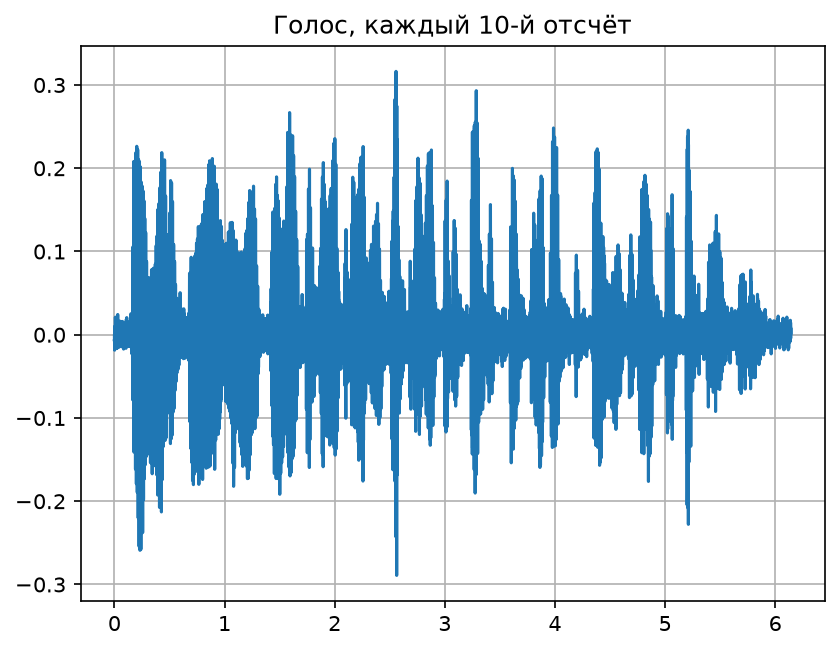
\includegraphics[width=0.8\textwidth]{c56_0.png}
\caption{Прореженный сигнал голоса (каждый 10-й отсчёт)}
\label{fig:c56_0}
\end{figure}

\subsubsection{Вывод}

Оригинал звучит чисто. Прореженный сигнал звучит глухо, с искажениями: мы оставили только 4410 отсчётов в секунду, а голосу нужно хотя бы 14 кГц (по теореме Котельникова). Это и есть последствия неверно выбранной частоты дискретизации.

\subsection{Задание 12}

Выполните прямое дискретное преобразование Фурье для оригинального звучания и для прореженного сигнала, выведите на график амплитудный спектр сигнала, определите его ширину.

\texttt{discrete\_fourier\_transform} считает за \texttt{N²} операций, а у записи сотни тысяч отсчётов. Поэтому для ускорения я взял готовую реализацую быстрого преобразования Фурье \texttt{np.fft.fft}.

Ширину спектра у голоса ровно до нуля не найти, поэтому считаем значимыми частоты, где амплитуда больше 1\% от самой большой.

\begin{lstlisting}[language=Python, caption={Функции расчёта спектра и его ширины}]
def get_spectrum(x: np.ndarray, fs: float) -> tuple[np.ndarray, np.ndarray]:
    N = len(x)
    # X = discrete_fourier_transform(x)
    X = np.fft.fft(x)
    half = N // 2 + 1  # без зеркальной части

    return np.arange(half) * (fs / N), np.abs(X[:half]) / N


def get_spectrum_width(freqs: np.ndarray, amp: np.ndarray, level: float = 0.01) -> float:
    return freqs[amp > level * amp.max()].max()
\end{lstlisting}

\begin{lstlisting}[language=Python, caption={Спектры и ширина спектров голоса}]
freqs_voice, amp_voice = get_spectrum(y_voice, Fs)
freqs_voice_down, amp_voice_down = get_spectrum(y_voice_down, Fs_down)

width_voice = get_spectrum_width(freqs_voice, amp_voice)
width_voice_down = get_spectrum_width(freqs_voice_down, amp_voice_down)

ic(width_voice)
ic(width_voice_down);
\end{lstlisting}

\begin{lstlisting}[language={}, numbers=none, backgroundcolor=\color{white}, caption={Результат выполнения: спектры и ширина спектров голоса}]
ic| width_voice: np.float64(7057.02903473535)
ic| width_voice_down: np.float64(2204.7557688757615)
\end{lstlisting}

\begin{lstlisting}[language=Python, caption={Построение спектра голоса (оригинал)}]
def draw_width_voice(ax: Axes) -> None:
    ax.axvline(width_voice, color="r", linestyle=":", label="ширина спектра")
    ax.legend()

show_plot(
    t=freqs_voice,
    func_val=amp_voice,
    title="Амплитудный спектр голоса, оригинал",
    on_axes=draw_width_voice,
)
\end{lstlisting}

\begin{figure}[H]
\centering
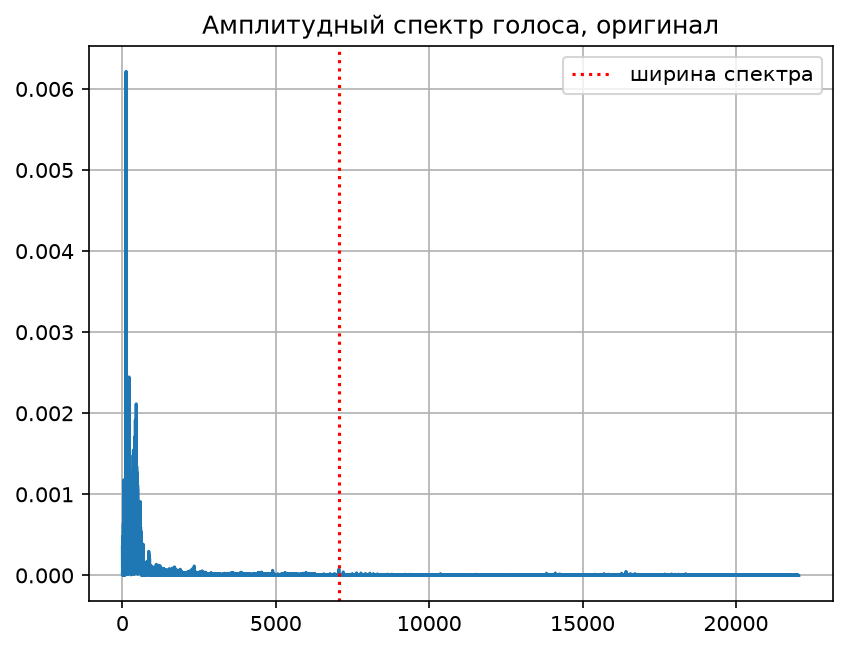
\includegraphics[width=0.8\textwidth]{c61_0.png}
\caption{Амплитудный спектр голоса, оригинал}
\label{fig:c61_0}
\end{figure}

\begin{lstlisting}[language=Python, caption={Построение спектра голоса (участок)}]
show_plot(
    t=freqs_voice[:len(freqs_voice)//20],
    func_val=amp_voice[:len(amp_voice)//20],
    title="Амплитудный спектр голоса, оригинал (до 20-й части)"
)
\end{lstlisting}

\begin{figure}[H]
\centering
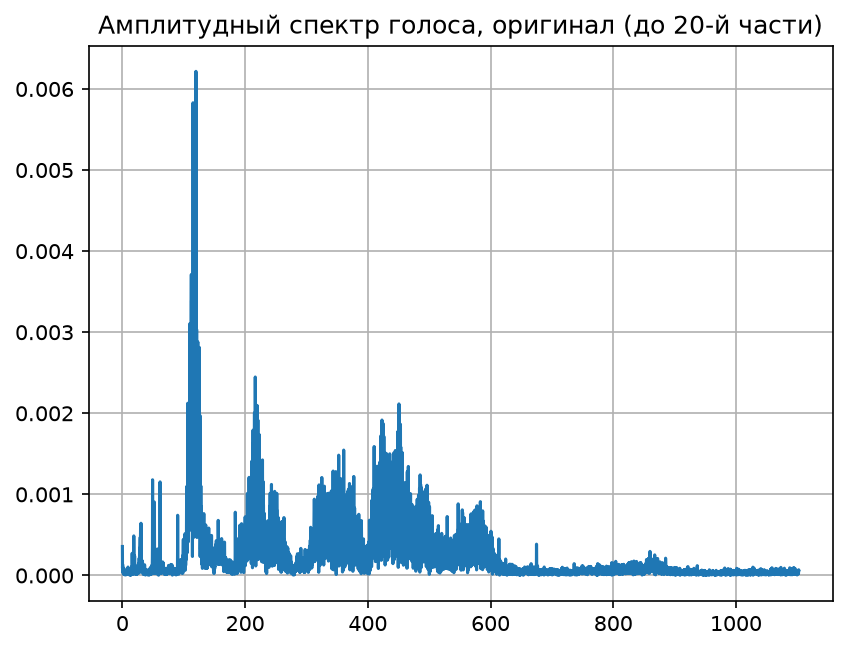
\includegraphics[width=0.8\textwidth]{c62_0.png}
\caption{Амплитудный спектр голоса, оригинал (первая двадцатая часть)}
\label{fig:c62_0}
\end{figure}

\begin{lstlisting}[language=Python, caption={Построение спектра голоса (прореженный сигнал)}]
def draw_width_voice_down(ax: Axes) -> None:
    ax.axvline(width_voice_down, color="r", linestyle=":", label="ширина спектра")
    ax.legend()

show_plot(
    t=freqs_voice_down,
    func_val=amp_voice_down,
    title="Амплитудный спектр голоса, каждый 10-й отсчёт",
    on_axes=draw_width_voice_down,
)
\end{lstlisting}

\begin{figure}[H]
\centering
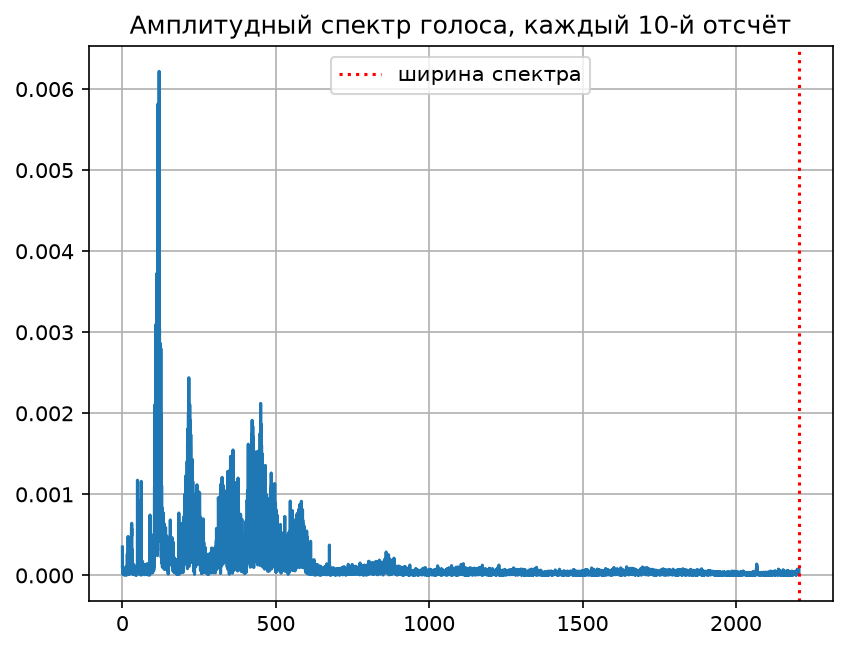
\includegraphics[width=0.8\textwidth]{c63_0.png}
\caption{Амплитудный спектр голоса, каждый 10-й отсчёт}
\label{fig:c63_0}
\end{figure}

\subsubsection{Вывод}

\begin{itemize}
\item Основная энергия голоса лежит в самых низких частотах (до нескольких сотен герц), дальше амплитуды спектра быстро падают.
\item У оригинала (44100 Гц) ширина спектра около 7 кГц, это согласуется с Audacity (задание 8).
\item После прореживания в 10 раз частота дискретизации стала 4410 Гц, и спектр обрезан на 2205 Гц (половина от новой частоты). Всё, что в голосе было выше, потерялось или "сложилось" с нижними частотами, поэтому звук стал глухим и "шакальным".
\end{itemize}

\subsection{Задание 13}

Оцените влияние разрядности АЦП на спектр сигнала. Для этого нужно написать функцию, которая бы округляла значения отсчетов сигнала, заданного в вашем варианте, до какого-то числа, определяемого разрядностью АЦП. Допустим если у АЦП всего 3 разряда, то диапазон возможных дискретных значений амплитуд временных отсчетов сигнала - это 0..7 (то есть, $7=2^3-1$). Все значения больше 7 округляются до 7. Для результирующего дискретного сигнала требуется выполнить прямое преобразование Фурье. Сравнить полученный спектр со спектром исходной синусоиды, отсчеты которой не подвергались квантованию по уровню. Вывести среднюю ошибку квантования для случаев, когда разрядность АЦП равна 3/4/5/6.

\subsubsection{Как работает квантование}

У АЦП с \texttt{bits} разрядами есть всего \texttt{2\textasciicircum{}bits} уровней (коды \texttt{0..2\textasciicircum{}bits - 1}). Наш сигнал бывает и отрицательным, поэтому сначала мы сдвигаем и растягиваем его так, чтобы он занял диапазон \texttt{0..2\textasciicircum{}bits - 1}, округляем до целого (это и есть код АЦП), всё, что вылезло за диапазон, обрезаем, и возвращаем обратно в исходный масштаб, чтобы можно было сравнивать с оригиналом.

Ошибка квантования - разница между исходным отсчётом и тем, что получилось после округления. Средняя ошибка - среднее модуля этой разницы.

\begin{lstlisting}[language=Python, caption={Квантование и средняя ошибка квантования}]
bits_list = [3, 4, 5, 6]
quantized = {bits: quantize(y_sampled, bits) for bits in bits_list}
quant_errors = {bits: np.mean(np.abs(y_sampled - quantized[bits])) for bits in bits_list}

ic(y_sampled.max())
ic(y_sampled.min())
ic("---------------------")

for bits in bits_list:
    ic(bits)
    ic(quant_errors[bits])
    ic("---------------------")
\end{lstlisting}

\begin{lstlisting}[language={}, numbers=none, backgroundcolor=\color{white}, caption={Результат выполнения: квантование и средняя ошибка квантования}]
ic| y_sampled.max(): np.float64(1.2588190451025218)
ic| y_sampled.min(): np.float64(-1.965925826289069)
ic| '---------------------'
ic| bits: 3
ic| quant_errors[bits]: np.float64(0.07986980422058564)
ic| '---------------------'
ic| bits: 4
ic| quant_errors[bits]: np.float64(0.036611652351682206)
ic| '---------------------'
ic| bits: 5
ic| quant_errors[bits]: np.float64(0.019374196344376298)
ic| '---------------------'
ic| bits: 6
ic| quant_errors[bits]: np.float64(0.011018439086669527)
ic| '---------------------'
\end{lstlisting}

\subsubsection{Спектры после квантования}

На каждом графике палочки - спектр квантованного сигнала, красные точки - спектр исходного.

\begin{lstlisting}[language=Python, caption={Спектры после квантования}]
def get_half_amp(x: np.ndarray) -> np.ndarray:
    return np.abs(discrete_fourier_transform(x))[:half] / len(x)

amp_origin = get_half_amp(y_sampled)

for bits in bits_list:
    def draw_origin(ax: Axes) -> None:
        ax.plot(freqs[:half], amp_origin, "ro", label="без квантования")
        ax.legend()

    show_plot(
        t=freqs[:half],
        func_val=get_half_amp(quantized[bits]),
        is_stem=True,
        title=f"Спектр, АЦП {bits} бит",
        on_axes=draw_origin,
    )
\end{lstlisting}

\begin{figure}[H]
\centering
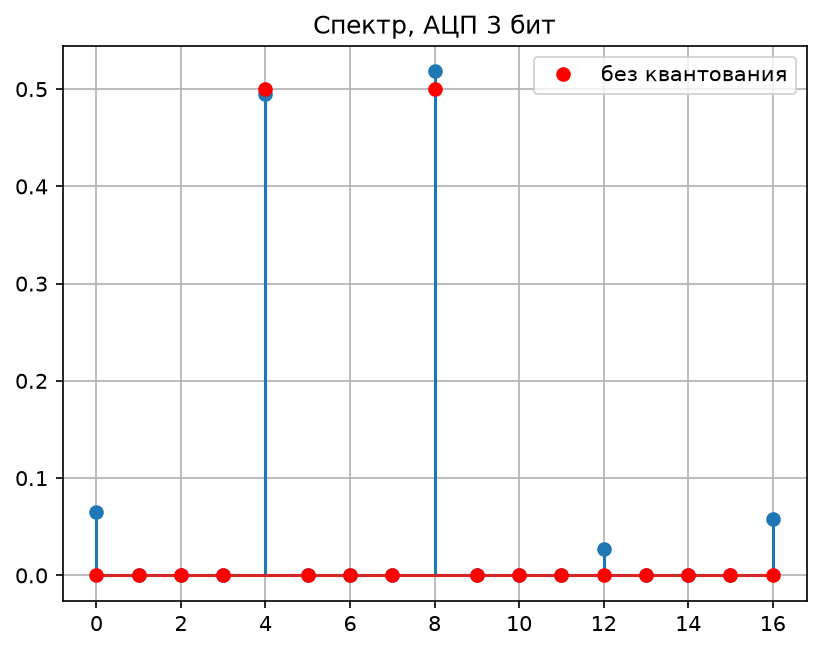
\includegraphics[width=0.8\textwidth]{c69_0.png}
\caption{Спектр квантованного сигнала, АЦП 3 бит}
\label{fig:c69_0}
\end{figure}

\begin{figure}[H]
\centering
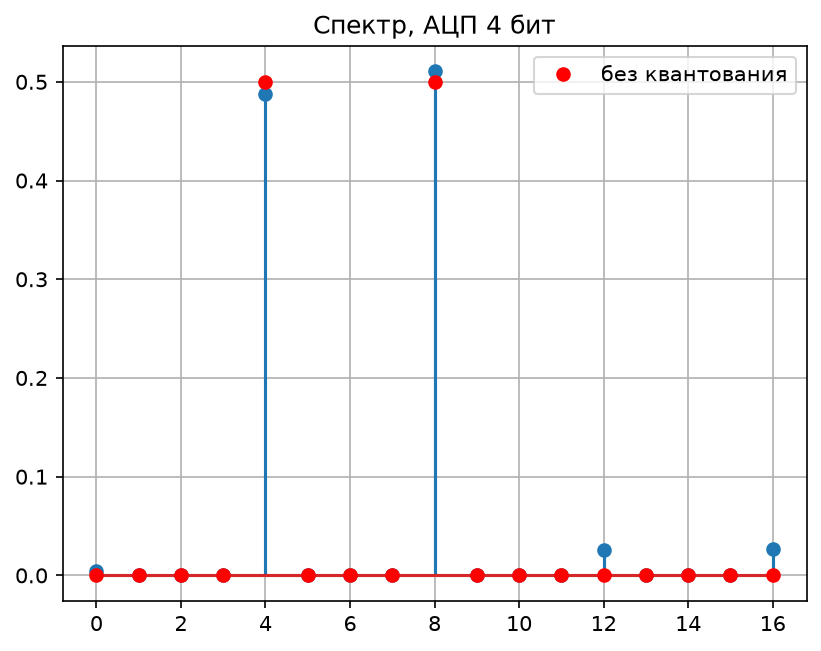
\includegraphics[width=0.8\textwidth]{c69_1.png}
\caption{Спектр квантованного сигнала, АЦП 4 бит}
\label{fig:c69_1}
\end{figure}

\begin{figure}[H]
\centering
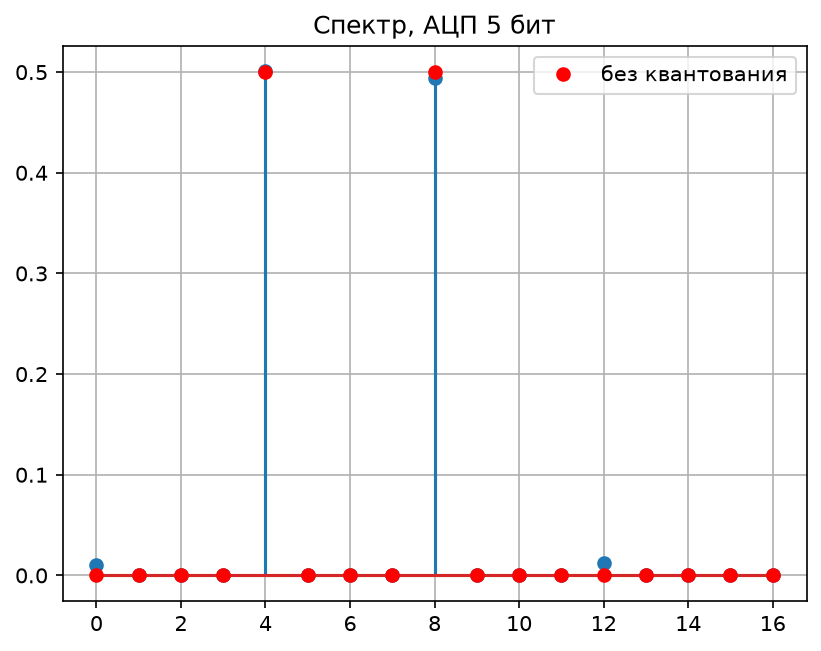
\includegraphics[width=0.8\textwidth]{c69_2.png}
\caption{Спектр квантованного сигнала, АЦП 5 бит}
\label{fig:c69_2}
\end{figure}

\begin{figure}[H]
\centering
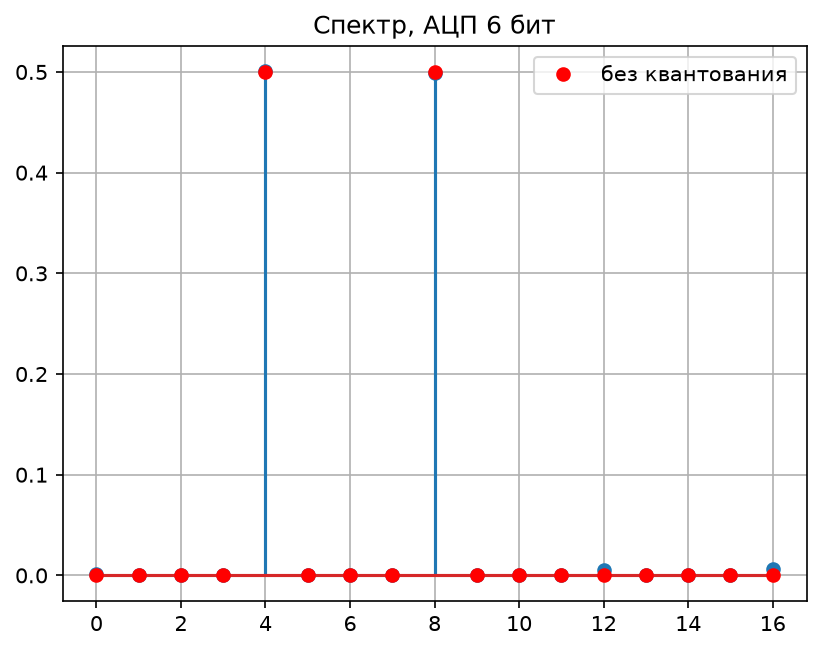
\includegraphics[width=0.8\textwidth]{c69_3.png}
\caption{Спектр квантованного сигнала, АЦП 6 бит}
\label{fig:c69_3}
\end{figure}

\subsubsection{Вывод}

Чем больше разрядов у АЦП, тем меньше средняя ошибка квантования (каждый лишний разряд примерно вдвое уменьшает её). На спектре ошибка выглядит как "шум" - маленькие палочки на частотах, где в исходном сигнале ничего нет. С ростом разрядности этот шум падает, а основные пики (4 и 8 Гц) почти не меняются.

\section{Ответы на контрольные вопросы}

\textbf{1) Для чего используются прямое и обратное преобразование Фурье?}

Прямое преобразование Фурье переводит сигнал из временного представления в частотное: показывает, из каких гармоник он состоит и какие у них амплитуды и фазы. Обратное делает наоборот: по частотному представлению восстанавливает сигнал во времени. Вместе они позволяют анализировать спектр сигнала, фильтровать его в частотной области и возвращаться обратно.

\textbf{2) Что такое ошибка квантования и дискретизации?}

Ошибка дискретизации возникает из-за того, что мы берём сигнал только в отдельные моменты времени. Если частота дискретизации слишком мала (не выполняется теорема Котельникова), часть информации теряется, а высокие частоты "складываются" с низкими. Ошибка квантования возникает из-за того, что амплитуду отсчёта приходится округлять до одного из $2^n$ уровней АЦП. Она не превышает половины шага квантования и тем меньше, чем больше разрядов у АЦП.

\textbf{3) Какое количество разрядов АЦП требуется, чтобы оцифровать голос?}

Для разборчивой речи (телефонная связь) хватает 8 разрядов. Для качественной записи обычно берут 16 разрядов: это 65536 уровней и динамический диапазон около 96 дБ.

\textbf{4) Как математически получить дискретные отсчеты непрерывного сигнала?}

Нужно взять значения непрерывной функции в моменты времени, кратные периоду дискретизации $T_s = 1/f_s$:

\begin{equation*}
x[n] = x(nT_s) = x\left(\frac{n}{f_s}\right),\quad n = 0, 1, 2, \dots
\end{equation*}

В коде это то же самое, что делать срез \texttt{y[::step]}.

\textbf{5) Какой спектр у периодического сигнала sin(10πt+π/2)?}

Так как $\sin(10\pi t + \pi/2) = \sin(2\pi \cdot 5 \cdot t + \pi/2) = \cos(10\pi t)$, это одна гармоника с частотой $f = 5$ Гц и амплитудой 1. Спектр состоит из одной линии на 5 Гц (в полном спектре ещё зеркальная линия на -5 Гц, каждая с амплитудой 0,5), начальная фаза $\pi/2$ у синусной формы записи.

\textbf{6) Что такое быстрое преобразование Фурье?}

Это алгоритм, который считает то же дискретное преобразование Фурье, но быстрее. Он использует повторяющиеся значения синуса и косинуса и группирует слагаемые с одинаковыми множителями. Вместо порядка $N^2$ операций нужно порядка $N \log_2 N$, а длина входа обычно равна степени двойки ($N = 2^k$). Поэтому БПФ используют в реальных модемах.

\textbf{7) Как определяется минимальная требуемая для оцифровки частота дискретизации сигнала?}

По теореме Котельникова: частота дискретизации должна быть строго больше удвоенной максимальной частоты в спектре сигнала,

\begin{equation*}
f_s > 2 f_{max}.
\end{equation*}


\section{Вывод}

В работе сгенерирован непрерывный сигнал варианта 5, представляющий собой сумму двух гармоник с частотами 4 и 8 Гц, поэтому максимальная частота его спектра равна 8 Гц. По теореме Котельникова частота дискретизации должна быть строго больше 16 Гц, при ровно 16 Гц отсчёты восьмигерцовой гармоники попадают в нули синуса и гармоника теряется. Выбрана частота 32 Гц: она в 4 раза больше максимальной частоты и нацело делит сетку из 1024 точек, поэтому отсчёты получаются равномерными.

Прямое дискретное преобразование Фурье для 32 отсчётов показало две значимые гармоники на частотах 4 и 8 Гц с амплитудой 0,5 каждая (вторая половина спектра - зеркальное отражение), амплитуды остальных частот порядка $10^{-16}$ и объясняются ошибками округления. Ширина спектра составила 8 Гц. Массив отсчётов в формате \texttt{float64} занимает 256 байт, массив спектра в формате \texttt{complex128} - 512 байт.

При соединении отсчётов линией восстановленный сигнал повторяет форму оригинала, но имеет вид ломаной, так как на период самой быстрой гармоники приходится всего 4 отсчёта, средняя ошибка составила 0,138. Увеличение частоты дискретизации в 4 раза (до 128 Гц) не изменило ширину спектра (8 Гц), так как новых частот в сигнале не появилось, но увеличило объём памяти в 4 раза (1024 байта) и уменьшило среднюю ошибку восстановления до 0,0082.

Анализ записи голоса в Audacity показал, что основная энергия сосредоточена в низких частотах, максимальная частота голоса около 6,2 кГц, следовательно, для оцифровки достаточно частоты дискретизации выше 12,4 кГц, например 16 кГц. Частота дискретизации записи, рассчитанная как число отсчётов, делённое на длительность, совпала со значением из файла и составила 44100 Гц. Ширина спектра оригинала при пороге 1\% от максимальной амплитуды около 7,06 кГц. После прореживания записи в 10 раз частота дискретизации стала 4410 Гц, спектр обрезан на частоте 2205 Гц, часть высоких частот потеряна или наложилась на низкие, поэтому звук стал глухим и искажённым.

Оценка влияния разрядности АЦП показала, что средняя ошибка квантования для 3, 4, 5 и 6 разрядов составляет 0,080, 0,037, 0,019 и 0,011 соответственно, то есть каждый дополнительный разряд уменьшает её примерно вдвое. На спектре ошибка квантования проявляется как шум малой амплитуды на частотах, которых нет в исходном сигнале, с ростом разрядности он уменьшается, а основные пики на частотах 4 и 8 Гц почти не меняются.

\section{Ссылка на репозиторий с кодом}

Исходный код работы доступен в репозитории: \url{https://github.com/Emeteil/mobile-communications-basics}.

\begin{figure}[H]
\centering

\includegraphics[width=0.4\textwidth]{qr_repo.png}
\caption{QR-код со ссылкой на репозиторий с кодом}
\label{fig:qr_repo}
\end{figure}

\end{document}
